\NeedsTeXFormat{LaTeX2e}

\documentclass[12pt]{article}
\usepackage[letterpaper,portrait, margin=1in]{geometry}
\usepackage{booktabs, pgfplots, bm, multirow, amsmath}
\pgfplotsset{width=11cm,compat=1.9}
\renewcommand{\arraystretch}{1.5}
\usepackage[colorlinks=true, allcolors=blue]{hyperref}
\usepackage{indentfirst}


\begin{document}
\begin{titlepage}

       %\vspace*{.5cm}
        \begin{center}
        \textbf{\huge PH-291 Physics Lab} \\ 
        \textbf{\Large Professor Corn-Agostini} \\ 
        \textbf{\Large Fall 2022} \\ 
        \vspace*{.5cm}  
        \textbf{\large Lab \# 1: Statistics of Measurement}
        \vspace{0.5cm}
        \end{center}
       
\noindent Your Name: Perla Berkovitz\\ \\
\noindent Your Lab Section: PH-291-E\\ \\
\noindent Your Lab Instructor: Professor Corn-Agostini\\ \\
\noindent Your Lab Partner's Name: Sharon Sitt\\ \\
\noindent Read and sign Academic Integrity Statement:\\

\noindent {\em I hereby attest that I have not given or received any unauthorized assistance on this assignment.}

    \begin{center}
    \line(1,0){300} \\
    Sign here
    \end{center}

\noindent\textbf{\large Grading Rubric} \\ \\
\renewcommand{\arraystretch}{1.5}
%\large
\begin{tabular}{|l|c|r|l|} 
\hline
 {\bf SECTION } & {\bf POINTS} & {\bf GRADE} & {\bf COMMENTS.................................}\\\hline 
Purpose & 1 & & \\\hline
Data & 3 & & \\\hline
Calculations  & 3 & & \\ \hline
Results & 3 & & \\\hline 
Conclusion & 1 & & \\ \hline
Answers & 4 & & \\\hline \hline 
{\em Total} & 15 & & \\ \hline
\end{tabular}
\end{titlepage}
\newpage
\tableofcontents
\newpage
\section{Purpose}
In this lab, various measurement devices are used to find the volume of a cylindrical disc and the density of an aluminum plate. A sample set is taken for each measurement to provide the most precise result given the uncertainty of each measurement device. While some devices might be more precise than others, all physical measurements have an innate degree of physical uncertainty. Calculating the uncertainty of the results allows the experimental data to have meaning. 
\newpage
\section{Data}
\begin{center}
    \begin{minipage}{.5\linewidth}
        \centering
        \begin{tabular}{|c | c|}
            \hline
            \textbf{Measurement} & \textbf{Thickness (mm)}  \\ \hline
            1 & 1.695 \\ 
            2 & 1.995 \\ 
            3 & 1.990  \\ 
            4 & 2.095 \\ 
            5 & 1.930 \\ 
            6 & 1.995 \\ \hline
            \multicolumn{2}{|c|}{\textbf{Instrumental Error:} 0.005 mm} \\
            \multicolumn{2}{|c|}{\textbf{Random Error:} 0.055 mm} \\
            \multicolumn{2}{|c|}{\textbf{Thickness:} $1.950\pm0.055$ mm} \\ \hline
        \end{tabular}
        \vspace{3mm}
        \\Table 1: Petri Dish Thickness
        \vspace{10mm}
    \end{minipage}%
    \begin{minipage}{.5\linewidth}
        \centering
        \begin{tabular}{|c | c|}
            \hline
            \textbf{Measurement} & \textbf{Thickness (mm)}  \\ \hline
            1 & 7.98 \\ 
            2 & 8.86 \\ 
            3 & 8.24  \\ 
            4 & 7.60 \\ 
            5 & 8.16 \\ 
            6 & 7.66 \\ \hline
            \multicolumn{2}{|c|}{\textbf{Instrumental Error:} 0.02 mm} \\
            \multicolumn{2}{|c|}{\textbf{Random Error:} 0.19 mm} \\
            \multicolumn{2}{|c|}{\textbf{Thickness:} $8.08\pm0.19$ mm} \\ \hline
        \end{tabular}
        \vspace{3mm}
        \\Table 2: Ring Diameter Without Liquid
        \vspace{10mm}
    \end{minipage} 
    \begin{tabular}{|c|c|}
        \hline
        \textbf{Measurement} & \textbf{Diameter (mm)} \\ \hline
        1 & 19.68 \\ 
        2 & 19.60 \\ 
        3 & 19.58 \\ 
        4 & 19.58 \\ 
        5 & 19.56 \\ 
        6 & 19.62 \\ \hline
        \multicolumn{2}{|c|}{\textbf{Instrumental Error:} 0.02 mm} \\
        \multicolumn{2}{|c|}{\textbf{Random Error:} 0.017 mm} \\
        \multicolumn{2}{|c|}{\textbf{Thickness:} $19.60\pm0.02$ mm} \\ 
        \hline
    \end{tabular}
    \vspace{3mm}
    \\Table 3: Ring Diameter With Liquid
    \begin{tabular}{|c|c c|}
    \hline
        \textbf{Measurement} & \textbf{Incident Angle} & \textbf{Refracted Angle} \\ \hline
        1 & $50.0\degree$ & $28.0\degree$ \\ 
        2 & $28.0\degree$ & $38.0\degree$ \\ 
        3 & $36.0\degree$ & $20.0\degree$ \\ 
        4 & $17.0\degree$ & $40.0\degree$ \\ 
        5 & $43.0\degree$ & $27.0\degree$ \\ 
        6 & $28.0\degree$ & $39.0\degree$ \\ \hline
        \multicolumn{3}{|c|}{\textbf{Instrumental Error:} $0.5\degree$} \\ \hline
    \end{tabular}
    \vspace{3mm}
    \\Table 4: Snell's Law
\end{center}
\newpage
\section{Calculations}
\textbf{\!\!\!\!\!\!\!\!\!\! 1. Volume of a cylindrical disc:}\[V_c=\pi\times\left(\frac{d}{2}\right)^2\times h\]
\begin{center}
    where \(r\) is the radius of the disc and \(h\) is the thickness of the disc.
    \[\textnormal{Sample Calculation: }V_c=\pi\times\left(\frac{3.9\textnormal{ cm}}{2}\right)^2\times0.35 \textnormal{ cm}=\boxed{4.18 \textnormal{ cm}^3}\]
\end{center}
\textbf{2. Volume of a rectangular object:}\[V_r=l\times w\times h\]
\begin{center}
    where \(l\) and \(w\) are the length and width respectively, and \(h\) is the thickness of the object.
    \[\textnormal{Sample Calculation: }V_r=4.15\textnormal{ cm}\times3.83\textnormal{ cm}\times0.31\textnormal{ cm}=\boxed{4.97 \textnormal{ cm}^3}\]
\end{center}
\textbf{3. Computing density:\[\rho=\frac{m}{V}\]}
\begin{center}
    where \(m\) and \(V\) are the mass and volume of each object.
    \[\textnormal{Sample Calculation: }\rho = \frac{10.5\textnormal{ g}}{4.18 \textnormal{ cm}^3}=\boxed{2.51\textnormal{ g}/\textnormal{cm}^3}\]
\end{center}
\textbf{4. Sample Mean:}\[\bar{x}=\frac{\sum\limits^{n}_{i=1}{x_i}}{n}\]
\begin{center}
    where \(x_i\) represents each value and \(n\) is the total number of entries
    \[\textnormal{Sample Calculation: }\bar{x}=\frac{\sum\limits^{20}_{i=1}x_i}{20}=\boxed{6.25 \textnormal{ mm}}\]
\end{center}
\textbf{5. Sample Standard Deviation:}\[S_x^2=\frac{1}{N_x-1}\sum^{N_x}_{i=1}(x_i-\bar{x})^2 \]
\begin{center}
    where \(S_x^2\) is the sample variance and \(S_x\) is the sample standard deviation for each sample set. \(N_x\) is the number of samples in the set. \\
    \[\textnormal{Sample Calculation: }S_x=\sqrt{\frac{\sum\limits^{20}_{i=1}(x_i-\bar{x})^2}{19}}=\boxed{0.66\textnormal{ mm}}\]
\end{center}
\textbf{6. Standard Deviation of the Mean (SDOM):}\[\sigma_x=\frac{S_x}{\sqrt{N_x}}\]
\begin{center}
    This also provides us with the random error of each sample set.\\
    \[\textnormal{Sample Calculation: }\sigma_x=\frac{0.66\textnormal{ mm}}{\sqrt{20}}=\boxed{0.15 \textnormal{ mm}}\]
\end{center}
\textbf{7. Test Statistic Value:}
\[t=\frac{\left|\bar{x}-\bar{y}\right|}{\sqrt{\sigma^2_{\bar{x}}+\sigma^2_{\bar{y}}}}\]
\[\textnormal{Sample Calculation: }t=\frac{|6.25-5.98|}{\sqrt{0.15^2+0.14^2}}=\boxed{1.32}\]
\textbf{8. Percent Improvement of Accuracy:}\[\%_{\textnormal{\,Improvement}} = 100-\frac{IE_{\textnormal{\,Vernier Caliper}}}{IE_{\textnormal{\,Linear Scale}}}\times 100 = 100- \frac{0.02}{0.5}\times 100 = \boxed{96\%}\]
\begin{center}
    where \textit{IE} refers to the instrumental error of each measurement instrument used.
\end{center}
\textbf{9. Error Propagation (Independent Variables):}
\[\delta f=\sqrt{\left(\frac{\partial f}{\partial x}\delta x\right)^2+\left(\frac{\partial f}{\partial y}\delta y\right)^2+\cdots+\left(\frac{\partial f}{\partial z}\delta z\right)^2}\]
\begin{center}
    where the variables $x,\,y,\,z$ are independent and used to determine the value of $f$. $\delta f$ provides the error of the function $f(x,\,y,\dots\,,z)$.
    \[\textnormal{Sample Calculation for $V_r$: }\delta V_r=\sqrt{\left(0.048\%\right)^2+\left(0.052\%\right)^2+\left(0.16\%)^2\right)}=\boxed{0.175\%} \]
\end{center}
\newpage
\section{Results}
\begin{center}
\begin{center}
    \begin{tabular}{|c|c|c|c|c|}
        \hline
        \textbf{Diameter (cm)} & \textbf{Thickness (cm)} & \textbf{Mass (g)} & \textbf{Volume ($\bm{\textbf{cm}^3}$)} & \textbf{Density (g/$\bm{\textbf{cm}^3}$)}  \\
        \hline
        3.9 & 0.35 & 4.18 & 10.5 & 2.51 \\ \hline
        3.95 & 0.35 & 4.29 & 10.5 & 2.45 \\ \hline
        3.9 & 0.35 & 4.18 & 10.6 & 2.54 \\ \hline
        3.95 & 0.3 & 3.68 & 10.5 & 2.86 \\ \hline
        3.9 & 0.35 & 4.18 & 10.6 & 2.54 \\ \hline
        3.95 & 0.35 & 4.29 & 10.5 & 2.45 \\ \hline
    \end{tabular}
\end{center}
\vspace{3 mm}
Table 13: Cylindrical Disk Results (Linear Scale)
\begin{center}
    \begin{tabular}{|c|c|c|c|c|}
        \hline
        \textbf{Diameter (cm)} & \textbf{Thickness (cm)} & \textbf{Mass (g)} & \textbf{Volume ($\bm{\textbf{cm}^3}$)} & \textbf{Density (g/$\bm{\textbf{cm}^3}$)}  \\
        \hline
        3.96 & 0.32 & 3.94 & 10.5 & 2.66 \\ \hline
        3.964 & 0.316 & 3.90 & 10.5 & 2.69 \\ \hline
        3.976 & 0.316 & 3.92 & 10.6 & 2.70 \\ \hline
        3.96 & 0.32 & 3.94 & 10.5 & 2.66 \\ \hline
        3.974 & 0.324 & 4.02 & 10.6 & 2.64 \\ \hline
        3.964 & 0.33 & 4.07 & 10.5 & 2.58 \\ \hline
    \end{tabular}
\end{center}
Table 14: Cylindrical Disk Results (Vernier Caliper)
\begin{center}
    \begin{tabular}{|c|c|c|c|c|}
        \hline
        \textbf{Diameter (cm)} & \textbf{Thickness (cm)} & \textbf{Mass (g)} & \textbf{Volume ($\bm{\textbf{cm}^3}$)} & \textbf{Density (g/$\bm{\textbf{cm}^3}$)}  \\
        \hline
        3.96 & 0.317 & 3.90 & 10.5 & 2.69 \\ \hline
        3.964 & 0.318 & 3.92 & 10.5 & 2.68 \\ \hline
        3.976 & 0.325 & 4.04 & 10.6 & 2.63 \\ \hline
        3.96 & 0.318 & 3.92 & 10.5 & 2.68 \\ \hline
        3.974 & 0.3205 & 3.98 & 10.6 & 2.67 \\ \hline
        3.964 & 0.317 & 3.91 & 10.5 & 2.68 \\ \hline
    \end{tabular}
\end{center}
Table 15: Cylindrical Disk Results (Micrometer)
\begin{center}
    \begin{tabular}{|c|c|c|c|c|}
        \hline
        \textbf{Diameter (cm)} & \textbf{Thickness (cm)} & \textbf{Volume ($\bm{\textbf{cm}^3}$)} & \textbf{Mass (g)} & \textbf{Density (g/$\bm{\textbf{cm}^3}$)}  \\
        \hline
        1.28\% & 14.29\% & 14.40\% & 0.48\% & 14.41\% \\ \hline
        1.27\% & 14.29\% & 14.40\% & 0.48\% & 14.41\% \\ \hline
        1.28\% & 14.29\% & 14.40\% & 0.47\% & 14.41\% \\ \hline
        1.27\% & 16.67\% & 16.76\% & 0.48\% & 16.77\% \\ \hline
        1.28\% & 14.29\% & 14.40\% & 0.47\% & 14.41\% \\ \hline
        1.27\% & 14.29\% & 14.40\% & 0.48\% & 14.41\% \\ \hline
    \end{tabular}
\end{center}
\vspace{3 mm}
Table 16: Cylindrical Disk Error Propagation (Linear Scale)
\begin{center}
    \begin{tabular}{|c|c|c|c|c|}
        \hline
        \textbf{Diameter (cm)} & \textbf{Thickness (cm)} & \textbf{Volume ($\bm{\textbf{cm}^3}$)} & \textbf{Mass (g)} & \textbf{Density (g/$\bm{\textbf{cm}^3}$)}  \\
        \hline
        0.05\% & 0.63\% & 0.63\% & 0.48\% & 0.79\% \\ \hline
        0.05\% & 0.63\% & 0.64\% & 0.48\% & 0.80\% \\ \hline
        0.05\% & 0.63\% & 0.64\% & 0.47\% & 0.79\% \\ \hline
        0.05\% & 0.63\% & 0.63\% & 0.48\% & 0.79\% \\ \hline
        0.05\% & 0.62\% & 0.62\% & 0.47\% & 0.78\% \\ \hline
        0.05\% & 0.61\% & 0.61\% & 0.48\% & 0.77\% \\ \hline
    \end{tabular}
\end{center}
Table 17: Cylindrical Disk Error Propagation (Vernier Caliper)
\begin{center}
    \begin{tabular}{|c|c|c|c|c|}
        \hline
        \textbf{Diameter (cm)} & \textbf{Thickness (cm)} & \textbf{Volume ($\bm{\textbf{cm}^3}$)} & \textbf{Mass (g)} & \textbf{Density (g/$\bm{\textbf{cm}^3}$)}  \\
        \hline
        0.05\% & 0.16\% & 0.17\% & 0.48\% & 0.51\% \\ \hline
        0.05\% & 0.16\% & 0.17\% & 0.48\% & 0.51\% \\ \hline
        0.05\% & 0.15\% & 0.17\% & 0.47\% & 0.50\% \\ \hline
        0.05\% & 0.16\% & 0.17\% & 0.48\% & 0.51\% \\ \hline
        0.05\% & 0.16\% & 0.17\% & 0.47\% & 0.50\% \\ \hline
        0.05\% & 0.16\% & 0.17\% & 0.48\% & 0.51\% \\ \hline
    \end{tabular}
\end{center}
Table 18: Cylindrical Disk Error Propagation (Micrometer)
\begin{center}
    \begin{tabular}{|c|c|c|c|c|c|}
        \hline
        \textbf{Length} & \textbf{Width} & \textbf{Thickness} & \textbf{Mass} & \textbf{Volume} & \textbf{Density}\\
        \textbf{(cm)} & \textbf{(cm)} & \textbf{(cm)} & \textbf{(g)} & \textbf{($\bm{\textbf{cm}^3}$)} & \textbf{(g/$\bm{\textbf{cm}^3}$)}\\
        \hline
        4.15 & 3.826 & 0.313 & 13.0 & 4.97 & 2.62\\ \hline
        4.15 & 3.824 & 0.322 & 13.0 & 5.11 & 2.54\\ \hline
        4.164 & 3.826 & 0.319 & 13.0 & 5.08 & 2.56\\ \hline
        4.168 & 3.824 & 0.3125 & 13.0 & 4.98 & 2.61\\ \hline
        4.166 & 3.824 & 0.3155 & 12.9 & 5.03 & 2.57\\ \hline
        4.156 & 3.824 & 0.3155 & 13.0 & 5.01 & 2.59\\ \hline
    \end{tabular}
\end{center}
Table 19: Rectangular Plate Results \\(Vernier Caliper (Length and Width) and Micrometer (Thickness))
\begin{center}
    \begin{tabular}{|c|c|c|c|c|c|}
        \hline
        \textbf{Length} & \textbf{Width} & \textbf{Thickness} & \textbf{Volume} & \textbf{Mass} & \textbf{Density}\\
        \textbf{(cm)} & \textbf{(cm)} & \textbf{(cm)} & \textbf{($\bm{\textbf{cm}^3}$)} & \textbf{(g)} & \textbf{(g/$\bm{\textbf{cm}^3}$)}\\
        \hline
        0.048\% & 0.052\% & 0.160\% & 0.175\% & 0.385\% & 0.422\% \\ \hline
        0.048\% & 0.052\% & 0.155\% & 0.171\% & 0.385\% & 0.421\% \\ \hline
        0.048\% & 0.052\% & 0.157\% & 0.172\% & 0.385\% & 0.421\% \\ \hline
        0.048\% & 0.052\% & 0.160\% & 0.175\% & 0.385\% & 0.423\% \\ \hline
        0.048\% & 0.052\% & 0.158\% & 0.174\% & 0.388\% & 0.425\% \\ \hline
        0.048\% & 0.052\% & 0.158\% & 0.174\% & 0.385\% & 0.422\% \\ \hline
    \end{tabular}
\end{center}
Table 20: Rectangular Plate Error Propagation \\(Vernier Caliper (Length and Width) and Micrometer (Thickness))  \\  
\begin{center}
    \begin{tabular}{|c|c|c|c|}
        \hline
        \textbf{Bottle \(\bm{\#}\)} & \textbf{\(\bm{\bar{x}}\) (mm)} & \textbf{\(\bm{S_x}\)} & \textbf{ \(\bm{\sigma_x}\)} \\
        \hline
         10 & 6.24 & 0.66 & 0.15 \\ \hline
         17 & 5.98 & 0.64 & 0.14 \\ \hline
         \multicolumn{4}{|c|}{\textbf{Test Statistic: }1.32} \\
         \hline
    \end{tabular}
\end{center}
Table 21: Statistics for Bottles 10 and 17
\end{center}
\begin{center}
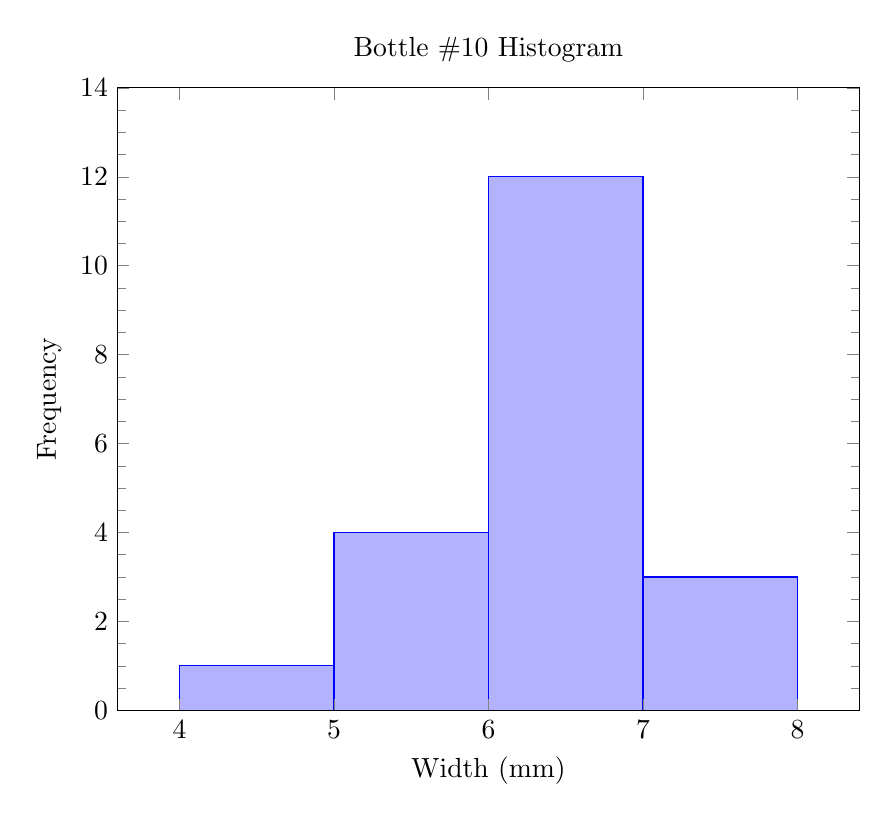
\begin{tikzpicture}
\begin{axis}[
    title={Bottle \(\#10\) Histogram},
    xlabel={Width (mm)},
    ylabel={Frequency},
    ymin=0, ymax=14,
    minor y tick num = 3,
    xtick=data,
    area style,
    ]
\addplot+[ybar interval,mark=no] plot coordinates { (4, 1) (5, 4) (6, 12) (7, 3) (8, 3) };
\end{axis}
\end{tikzpicture}
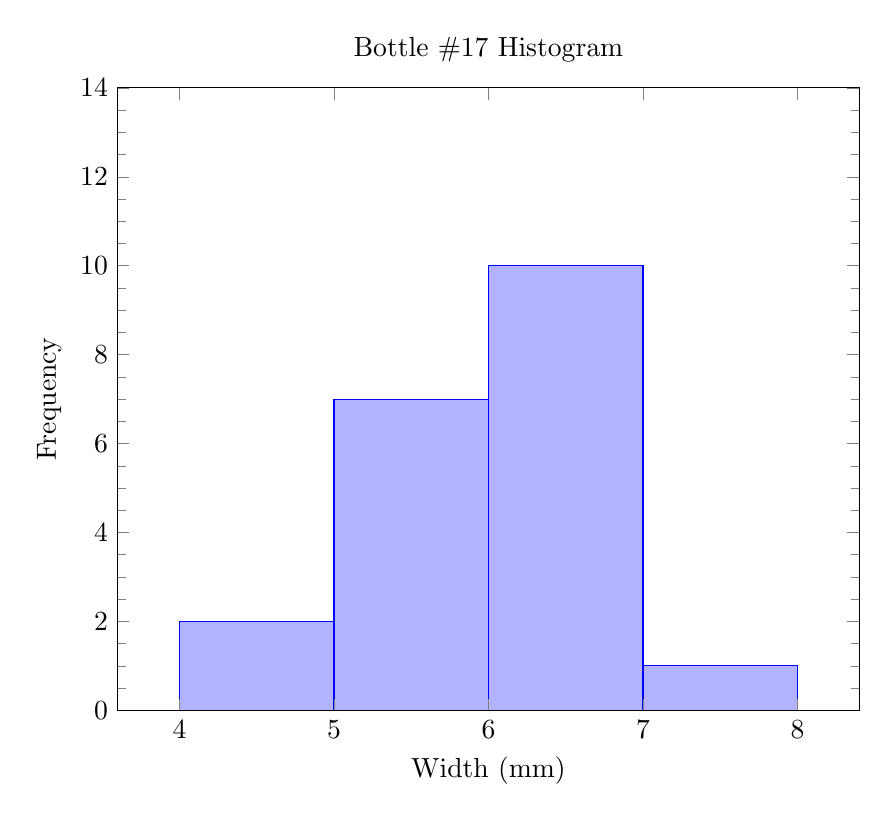
\begin{tikzpicture}
\begin{axis}[
    title={Bottle \(\#17\) Histogram},
    xlabel={Width (mm)},
    ylabel={Frequency},
    ymin=0, ymax=14,
    minor y tick num = 3,
    xtick=data,
    area style,
    ]
\addplot+[ybar interval,mark=no] plot coordinates { (4, 2) (5, 7) (6, 10) (7, 1) (8, 1) };
\end{axis}
\end{tikzpicture}
\end{center}
\newpage
\section{Conclusion}
In the first part of the experiment, the volume of a cylindrical disc was calculated using measurements taken by a linear scale and then by a vernier caliper. The vernier caliper was a more accurate measurement device than the linear scale due to its lower instrumental error. As expected, the overall error in calculating the volume, which included both the instrumental and random error, was reduced relative to the change in instrumental error. The calculated volume using measurements from the linear scale had an average error of 14.8\%, while the measurements from the vernier calipers provided an error of 0.63\%, which shows a 95.8\% decrease in error.
\par Aluminum alloy 6061 is known to have a density of 2.7 g/cm$^3$, which corresponds to the calculated densities of both the rectangular and cylindrical plates. The density value calculated using measurements from the micrometer was 2.67 $\pm$ 0.01 g/cm$^3$, which is only 1.1\% lower than the known value. The slight difference in calculated densities can be attributed to instrumental error, random error, and imperfections in the plates. The vernier calipers and the micrometer are made of steel, which is significantly harder than aluminum. If the measurement devices were clamped too tightly around the plate, they may eat into the material and provide inaccurate results. 
\par The final part of the experiment compares the dimensions of acrylic pieces in two separate bottles. The null hypothesis states that the averages lengths of pieces in each bottle will be equal. The histograms for each bottle don't appear to follow a particular distribution. In bottle 10, the average length was 6.25 $\pm$ 0.005 mm. In bottle 17, the average length was 5.98 $\pm$ 0.005 mm. These numbers do not initially appear to be equal, however by using the t-test, a p-value of 40.9\% was obtained which allows us to fail to reject the null-hypothesis.
\newpage
\section{Discussion Questions}
\begin{enumerate}
    \item Compare the two error values. Did the better instrument produce a corresponding reduction in error value? (For example, if the better instrument had a 20\% less instrumental error, did your final result show a 20\% reduction in error?) If not, why?\\\\
    The better instrument, being the one with a greater accuracy, produced a correspondingly lower error. For example, when comparing the calculated volumes using the linear scale and the vernier calipers, the error decreased by about 96\%, which is the same as the decrease in instrumental error.\\
    \item Do the density values agree with one another and the standard value? (Remember, you will have to include the uncertainties when you answer this question).\\\\
    The standard value of the density of Aluminum alloy 6061 is 2.7 g/cm$^3$. The density calculated using the linear scale measurement of the cylindrical disc was 2.56 $\pm$ 0.4 g/cm$^3$. The density calculated from vernier caliper measurements of the cylindrical disc was 2.66 $\pm$ 0.02 g/cm$^3$. The measurements of the disc with the micrometer provided a density of 2.67$\pm$ 0.01 g/cm$^3$. Finally, the measurements of the rectangular plate provided a density of 2.58 $\pm$ 0.01 g/cm$^3$. These experimental values agree with one another within the error range, but are slightly lower than the standard value.\\
    \item Comment if your data sets follow a normal distribution (the table in the margin shows what a normal distribution should be like).\\\\
    The data from bottles 10 and 17 does not follow a normal distribution. Both histograms do not seem to follow any specific distribution pattern, which corresponds to variety of lengths in each bottle.\\
    \item Using the t value decide if your data supports the null hypotheses at the 5\% significance level.\\\\
    The expected t value at 5\% significance level with 19 degrees of freedom is 1.729. The calculated value was 1.32. The p-value, which is the difference between the two t-values, is 0.409 (40.9\%) which means that the p-value supports the null hypothesis.
\end{enumerate}
\end{document}